\chapter{Design of Power Elites Web App}
\label{chapwebapp}

In the present chapter, we dissect our system bit by bit and describe each component in detail. We have already described how our data is integrated from different data sources, and also how our ER system works. Here we describe the wiki and the web application that uses all those features. It is important to note that that our main goal while designing the web application (and the entire system) was to reduce manual work of the verifier - so a lot of brainstorming and design changes went in that direction. Any feature or performance improvement in the verification process makes life easy for the verifier. The system has been designed to be able to crowd-source the verification process. \\

Another key point which we have kept in mind while building the system is to make the 
data-gatherers' task hassle-free - that they should universally be able to communicate with the system. Towards this effect they should also be able to keep track of their data, and update their old data as well. We have already described how we achieve this using JSON and REST over a Neo4j back-end which we call crawl data-store. We have already described how separation of concerns further help in achieving this as the crawled-data is well separated in crawl data store. \\

\section{Terminology}

\begin{figure}[H]
\begin{center}  
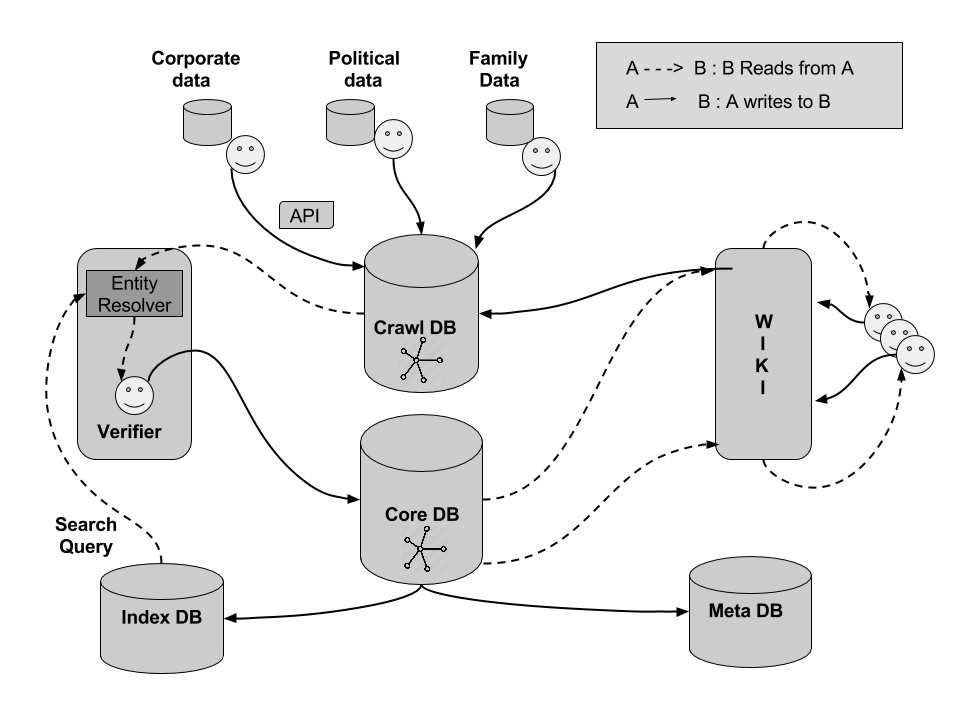
\includegraphics[width=1\textwidth]{system} 
\caption{System Design}
\label{fig:system}
\end{center}
\end{figure}

The detailed design of the system can be seen in \ref{fig:system}. We formally define the terminology about the actors and the system components here:

\begin{enumerate}
    
    \item \textbf{Data-Gatherer:} An authorized individual or a group of individuals who crawl linked data from different sources. This data can be about entities and relations that belong to a domain supported by our system: political, corporate, sports, bureaucratic, etc. A data-gatherer can use their API-token to push data to our crawl data store using JSON payload.

    \item \textbf{Crawl Data Store:} The Neo4j data store which stores all non-verified, non-resolved data that data-gatherers push into the system. All data from here is first verified and resolved.

    \item \textbf{Resolver:} A tool that searches over indexed graph data to suggest possible matching entities for a given entity. ER mechanism has been described in Section \ref{dataer}. A resolver in essence in our system suggests the probable matches but does not resolve.

    \item \textbf{Verifier:} An authorized person who matches an entity against a possible list of suggestions by the resolver. The only human element on which the system is dependent to be able to push correct data to the core data store.

    \item \textbf{Core Data Store:} The Neo4j data store which stores all verified, resolved data that data-gatherers push into the system.  This basically represents our knowledge base - an integration of data from different sources.

    \item \textbf{Registered User:} An authorized user who can use wiki to suggest changes to an entity or a relation in the core data store. All these changes are directed to crawl data store. 

    \item \textbf{Wiki:} Part of the web app, where registered users can edit or add information to the core data store.

    \item \textbf{Meta-DB:} MySQL back-end which stores provenance of any info added or changed in the core data store.

    \item \textbf{Index-DB:} MySQL back-end which stores condensed information (and connected information) of all the entities in the core data store. Apache Solr runs on top of it to index this information to speed-up the resolution process. 

    \item \textbf{Admin:} The user with all the privileges in the system - can delete all indexes, refresh all indexes, see which user/verifier contributed most to the system, change role of a user, etc.

    \item \textbf{End user:} Non-authorized users that can access information through the web app. They cannot make or suggest any changes to the core data store.

    \item \textbf{Role:} All the authorized users in the system are given a role. The roles are in a scoping fashion. The role order from the top is as follows: Admin, Verifier, Crawler, Registered User, End User.  

\end{enumerate}

% We have described the tech used in the system in the appendix section. [TODO: did we??]



\section{Data Gatherer}

The use case diagram for data-gatherer is shown in Figure \ref{fig:gatherer}.

\begin{figure}[H]
\begin{center}  
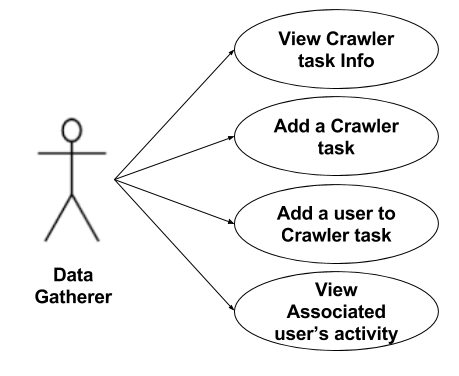
\includegraphics[scale=0.3]{gatherer} 
\caption{Use cases for Data Gatherer}
\label{fig:gatherer}
\end{center}
\end{figure}


\subsection{Task creation}
A group of data-gatherers are assigned a unique task identifier when they create a task for their crawled data (Figure \ref{fig:taskcreate}). This helps in separating the data from different tasks, due to which the crawl data-store has different disconnected subgraphs. The data-gatherers can keep track of their pushed info using the task identifiers (Figure \ref{fig:tasksall}). Each node and each relation for a task has to be uniquely named by the data-gatherers relative only to their task id.


\begin{figure}[H]
\begin{center}  
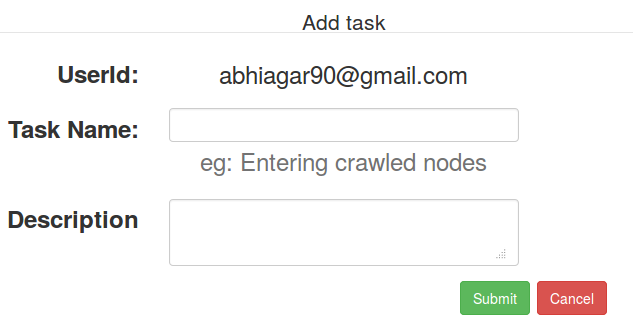
\includegraphics[width=0.6\textwidth]{taskcreate} 
\caption{Creating tasks for a data-gathering group}
\label{fig:taskcreate}
\end{center}
\end{figure}


\begin{figure}[H]
\begin{center}  
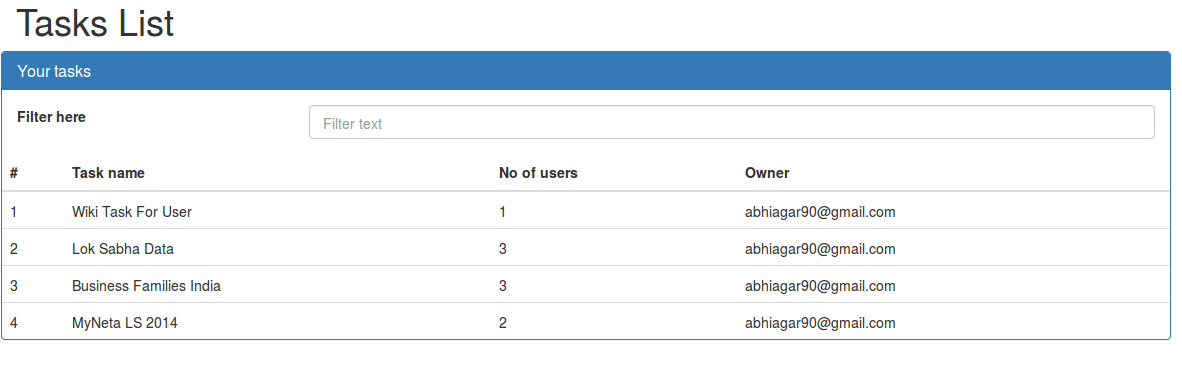
\includegraphics[width=1\textwidth]{tasksall} 
\caption{Information about a task}
\label{fig:tasksall}
\end{center}
\end{figure}


\subsection{User Addition}
By default when a task is created, the owner is automatically added as one the users of the created task.
He can add more users to the task which will allow those users to be able to push data specific to that task (Figure \ref{fig:taskadduser}).

\begin{figure}[H]
\begin{center}  
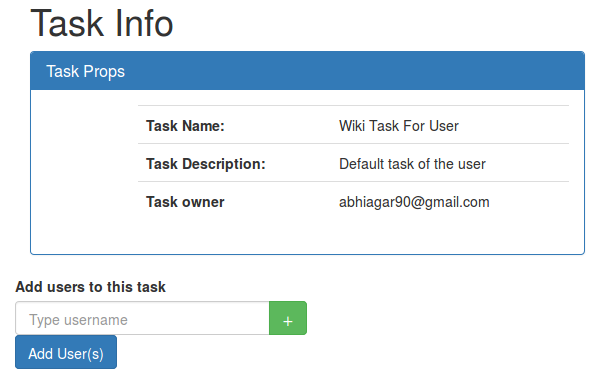
\includegraphics[width=0.7\textwidth]{taskadduser} 
\caption{Adding users to a task}
\label{fig:taskadduser}
\end{center}
\end{figure}


\subsection{Authorization \& POST API}
Every authorized user in the system is given an api-token at the time of sign-up. An api request is authorized if userid and api-token are provided correctly. For pushing data to the system using a valid api-request, JSON has been employed as the payload. The structure has been described in Section \ref{dataint}. To push the JSON to the system, the API request is described in Table \ref{tab:postjson}.

\begin{table}[H]
\centering
\caption{Request API: /apis/postgraph/?userid=$\langle userid \rangle$\&token=$\langle tokenid \rangle$}
\label{tab:postjson}
\begin{tabular}{ll}

\textbf{URL Parameters} & userid, token                              \\

\hline

\textbf{Headers}        & Content-Type : application/json            \\

\hline

\textbf{Payload}        & JSON                                       \\

\hline

\textbf{JSON VARS}      & taskid, userid, token, entities, relations \\
\hline

\textbf{HTTP-METHOD}    & POST      \\
\hline                                

\end{tabular}
\end{table}

\subsection{JSON Response}
If request is authorized and JSON is as per our convention, then the data is pushed to the crawl data-store. Validations before the push happen as described in the \ref{dataint}. The response is almost identical copy of the request JSON, including the meta-data. All the meta-data has been marked with a beginning and an ending underscore as shown in \ref{jsonresponse} \\


\label{jsonresponse}
\begin{lstlisting}[language=json,firstnumber=1]
"16": {
      "labels": [
        "person",
        "entity",
        "indian",
        "politician"
      ],
      "properties": {
        "_crawl_en_id_": "en_7_16",
        "_fetchdate_": 1466781745,
        "_nodenumber_": 16,
        "_pushdate_": 1467056465.732715,
        "_pushedby_": "mridul.goel53@gmail.com",
        "_sourceurl_": "https://www.wikipedia.org/",
        "_taskid_": 7,
        "name": "Akhilesh Yadav"
      }
    }
\end{lstlisting}



\section{Resolver and verifier}

\begin{enumerate}

\item \textbf{Use Case:} The use case diagram for verifier is shown in Figure \ref{fig:verifier}


\begin{figure}[H]
\begin{center}  
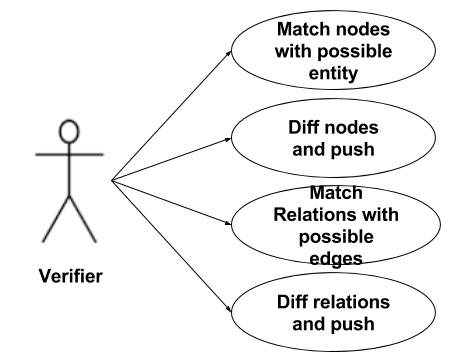
\includegraphics[scale=0.3]{verifier} 
\caption{Use cases for Verifier}
\label{fig:verifier}
\end{center}
\end{figure}
 
\item \textbf{Resolution:} Every node in the crawl data-store has to be resolved to a node (existing or new) in the core data-store. To resolve an entity is to provide it with a uuid. Similarly for relations, a relid is provided. This is achieved when a verifier picks up an object during match (Figure \ref{fig:match}) from the possible list of objects suggested by the resolver. Diff view (Figure \ref{fig:diff}) aids the verifier to granularly look at new labels, new properties and conflicting properties (shown with differentiating colors).

\begin{figure}[H]
\begin{center}  
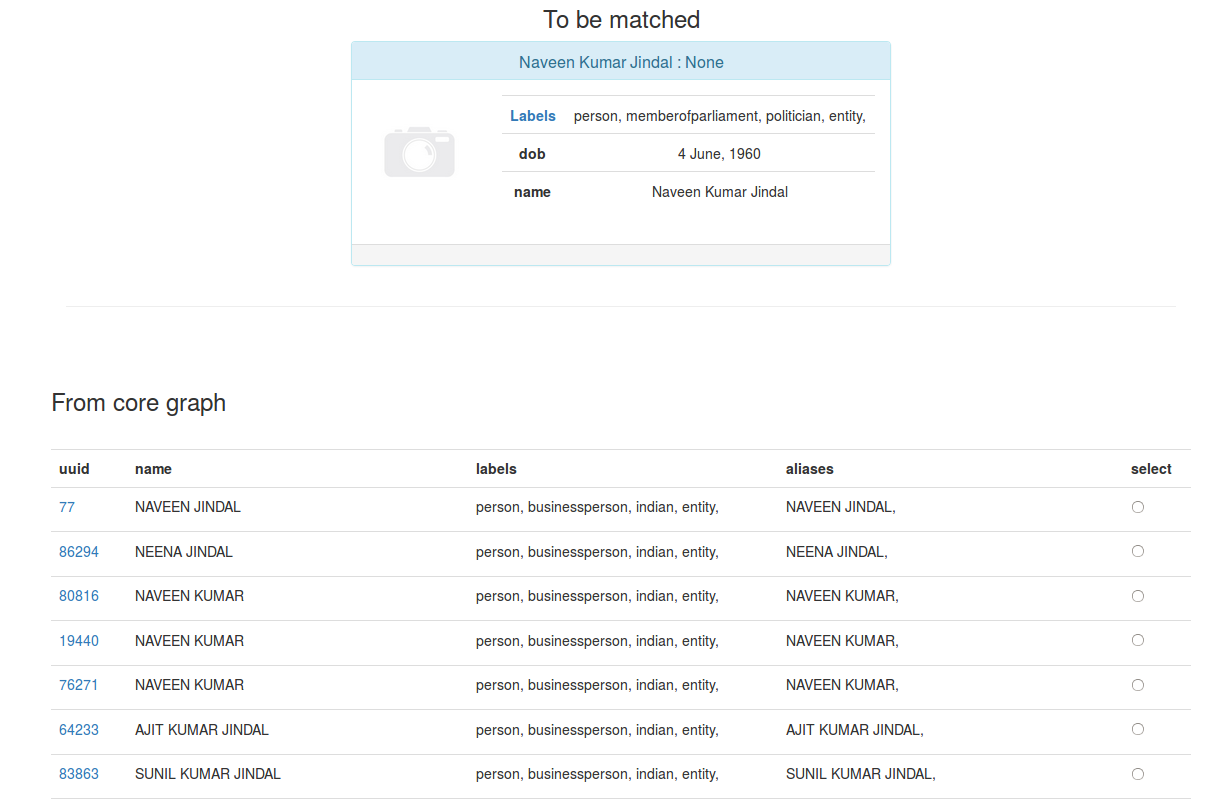
\includegraphics[width=1\textwidth]{match} 
\caption{The match-view in verification task}
\label{fig:match}
\end{center}
\end{figure}

\begin{figure}[H]
\begin{center}  
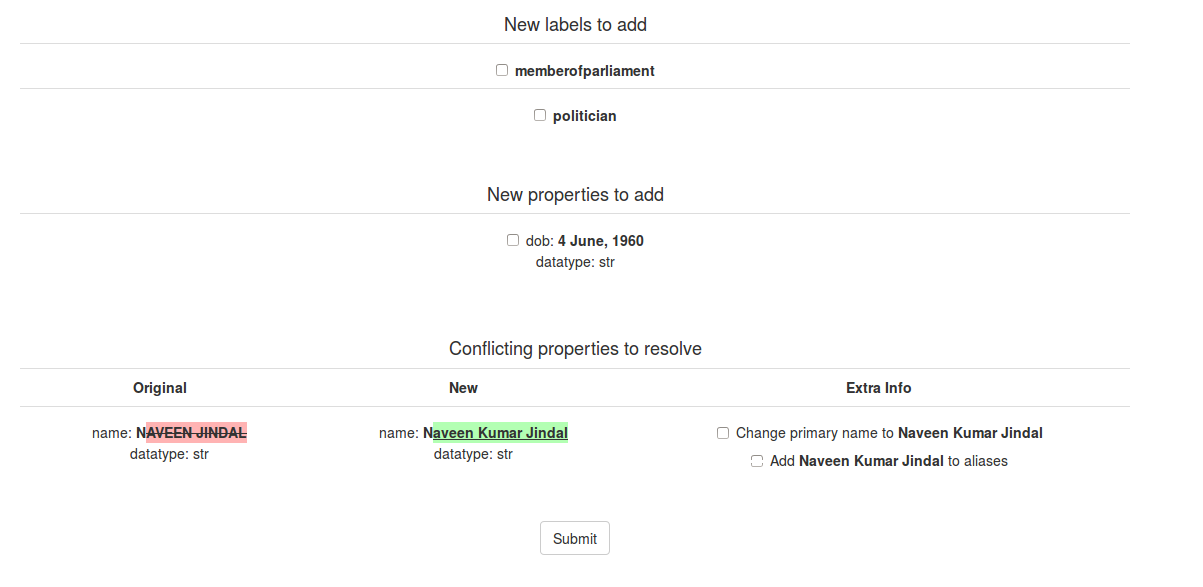
\includegraphics[width=1\textwidth]{diff} 
\caption{The diff-view in verification task}
\label{fig:diff}
\end{center}
\end{figure}

\item The key idea is to design views to facilitate the verification task for the verifiers, to help them in focusing on investigating the new information in the least possible time. 

\item \textbf{Selection algorithm:} A selection algorithm picks up the next nodes or relations to resolve. When left with no choice, it picks up the highest degree node, else the node that has the highest number of connected resolved nodes is picked.

\item \textbf{Validations}: Robust validations have been used on match and diff view to ensure that nothing inconsistent happens to the core data-store. Option to resume an on-going task, clear current session, release all locks have also been provided (Figure \ref{fig:session}).

\begin{figure}[H]
\begin{center}  
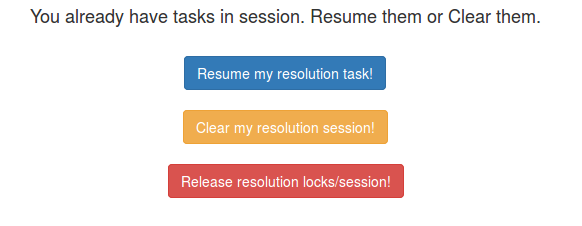
\includegraphics[width=0.7\textwidth]{session} 
\caption{Session Handling during Verification task}
\label{fig:session}
\end{center}
\end{figure}


\item \textbf{Parallelization:} A graph object selected during a verifier's session is locked for some time to let the selection algorithm know of it's status, this way the selection algorithm picks up another potential node for a new user.

\item \textbf{Jaro:} Provision for running jaro on fetched entities from Apache Solr has been provided in the match view. In practice, phonetic has been seen to be do very well for names we have encountered. We have kept this feature extensible in the sense if some other algorithms need to be tested for the task.

\item \textbf{Multi valued-properties:} Extensive care has been taken to incorporate multi-valued property for nodes and relationships. During the diff task, a merge request on the property can result in converting the original value of the property to a multi-valued one. 

\end{enumerate}




% \subsection{Guideline for the verification task}

% a mini-guide to manual verification -- reema sarkar -- [an image]
% very imp as only write happens through verifier
% shortest path
% expand on nodes in neo4j yuvraj singh a falase case can describe
% examples of connection --- between sons etc. 
% screenshots verifier \\
 

\section{Authorized User and Wiki}

\begin{enumerate}

\item \textbf{Use Case:} Use case diagram for authorized users is shown in Figure \ref{fig:registereduser}.

\begin{figure}[H]
\begin{center}  
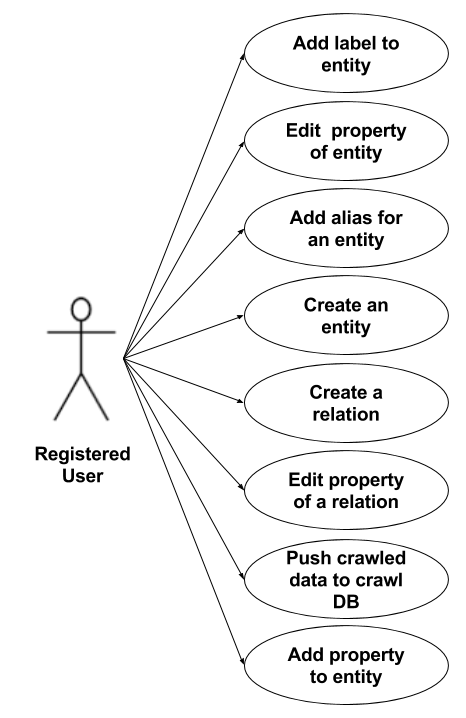
\includegraphics[scale=0.4]{registereduser} 
\caption{Use cases for registered users.}
\label{fig:registereduser}
\end{center}
\end{figure}

\item \textbf{Wiki:} Authorized users can access the wiki to edit entities and relationships in the core data-store. All these edits are first sent to the crawl data-store in the same fashion as any JSON from a data-gatherer is handled. This way all changes in the system occur through the verification process so that the core data-store is free of any noise or redundancy. 


\item \textbf{Wiki features:} Wiki can be accessed to add a new node, add a  new relation (Figure \ref{fig:addrel}),  edit an existing node, add a new label (Figure \ref{fig:addlabel}), edit an existing relation. A user can add as many properties to the entity/relationship as possible (Figure \ref{fig:oldprops}). Certain properties that can be potential candidates for addition are also suggested in the edit view (Figure \ref{fig:oldprops}). 

\begin{figure}[H]
\begin{center}  
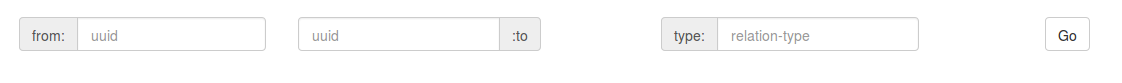
\includegraphics[width=1\textwidth]{addrel} 
\caption{Add relation between two entities}
\label{fig:addrel}
\end{center}
\end{figure}


\begin{figure}[H]
\begin{center}  
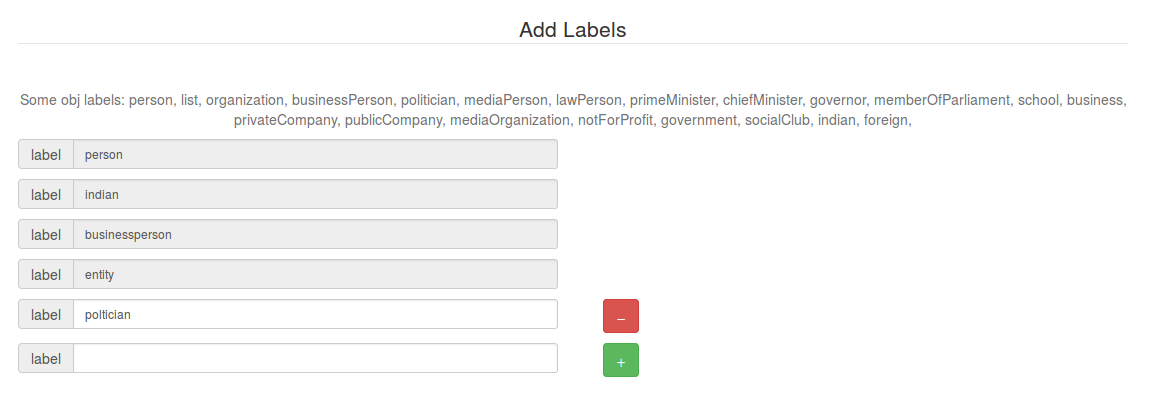
\includegraphics[width=1\textwidth]{addlabel} 
\caption{Add new labels to a node}
\label{fig:addlabel}
\end{center}
\end{figure}

\begin{figure}[H]
\begin{center}  
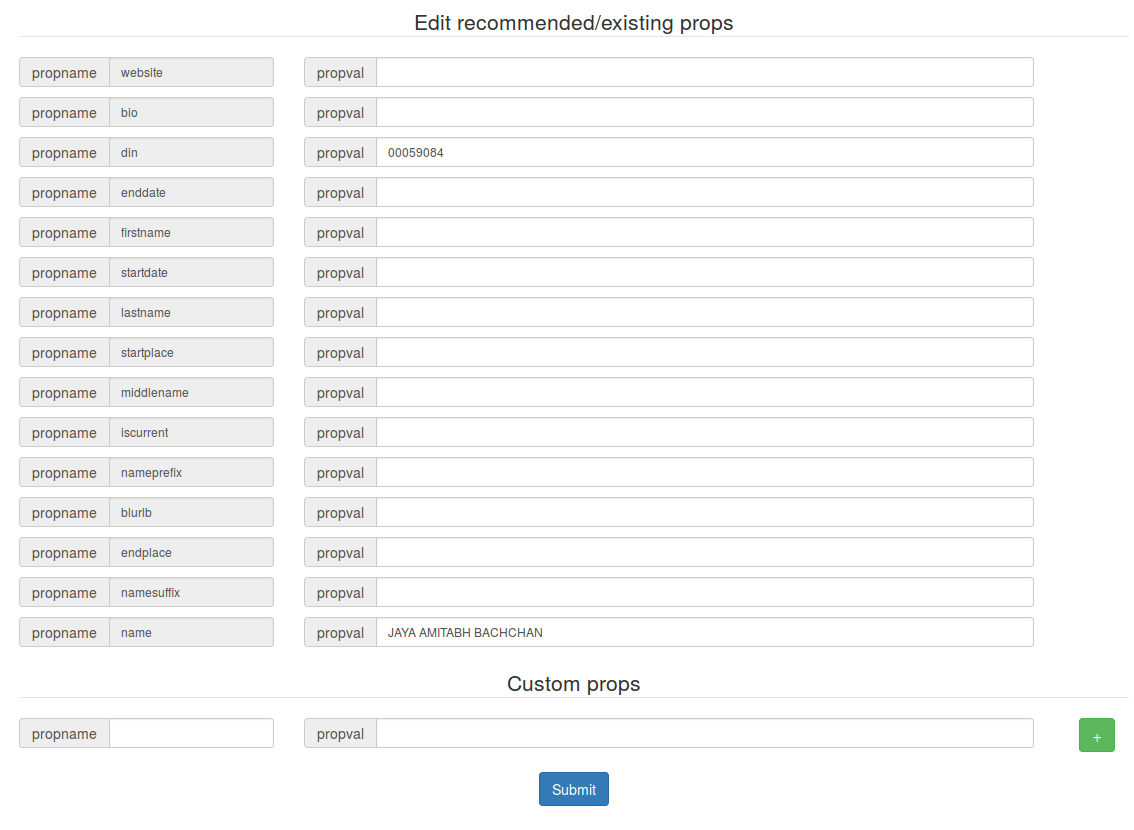
\includegraphics[width=1\textwidth]{oldprops} 
\caption{Edit existing properties/Add recommended properties}
\label{fig:oldprops}
\end{center}
\end{figure}



\end{enumerate}


\section{Provenance}
\label{sectionprov}

\begin{enumerate}

\item \textbf{Accountability:} We felt the need to maintain every granular detail about any change in the core data store. Thus, a label addition, a property change, a property addition, all need to be accounted for - who pushed the change, when was it pushed, when was the data collected by the data-gatherer, who verified the change, the source-url for the new information, etc.

\item \textbf{Meta-DB:} All this meta-data is stored on a dedicated MySQL back-end that is updated as soon as a new updation is approved by the verifier. 

\item \textbf{History:} A history feature on the web application for each entity and for each relation helps an end user to see our provenance meta-data. The same is better viewed in Figure \ref{fig:prov1} and Figure \ref{fig:prov2}.

\begin{figure}[H]
\begin{center}  
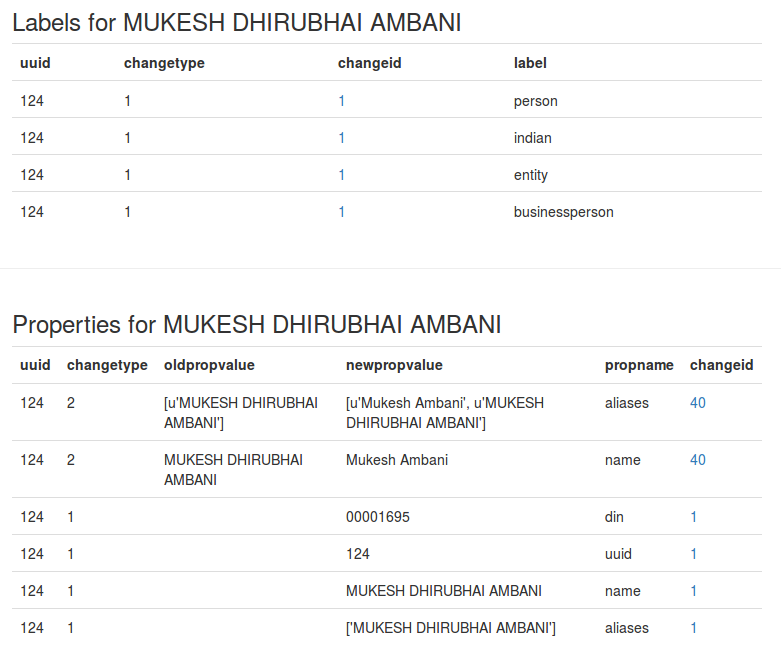
\includegraphics[scale=0.4]{prov1} 
\caption{Every change is attributed to a change ID}
\label{fig:prov1}
\end{center}
\end{figure}


\begin{figure}[H]
\begin{center}  
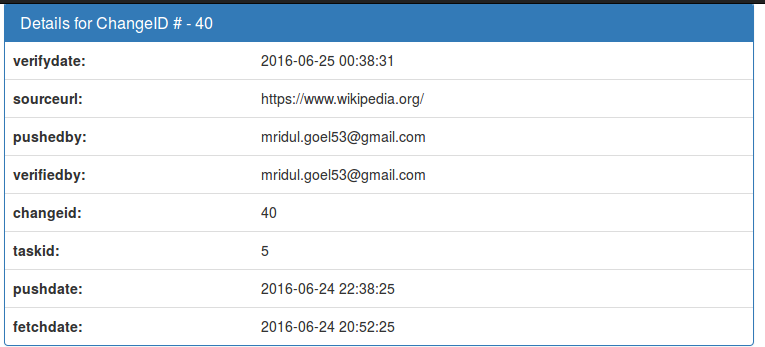
\includegraphics[scale=0.5]{prov2} 
\caption{Every change has associated meta-data}
\label{fig:prov2}
\end{center}
\end{figure}


\end{enumerate}





\section{End user}

\begin{enumerate}

\item \textbf{Use Case:} Use case diagram for not logged-in end users is shown in Figure \ref{fig:enduser}.

\begin{figure}[H]
\begin{center}  
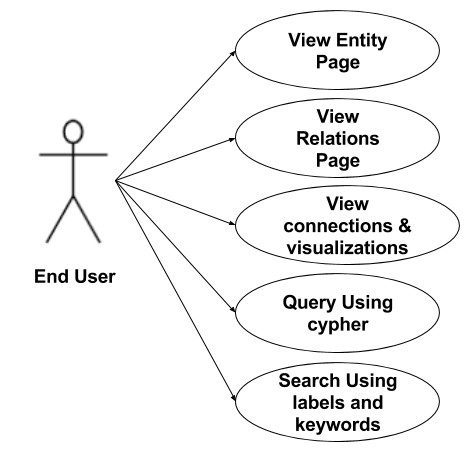
\includegraphics[scale=0.3]{enduser} 
\caption{Use cases for End User}
\label{fig:enduser}
\end{center}
\end{figure}




\item \textbf{Search:} End user can search for entities in our core data store. The search is powered by Apache Solr and uses double metaphone. The search can be filtered on labels and keywords. An actual search query is shown in Figure \ref{fig:endsearch} 

\begin{figure}[H]
\begin{center}  
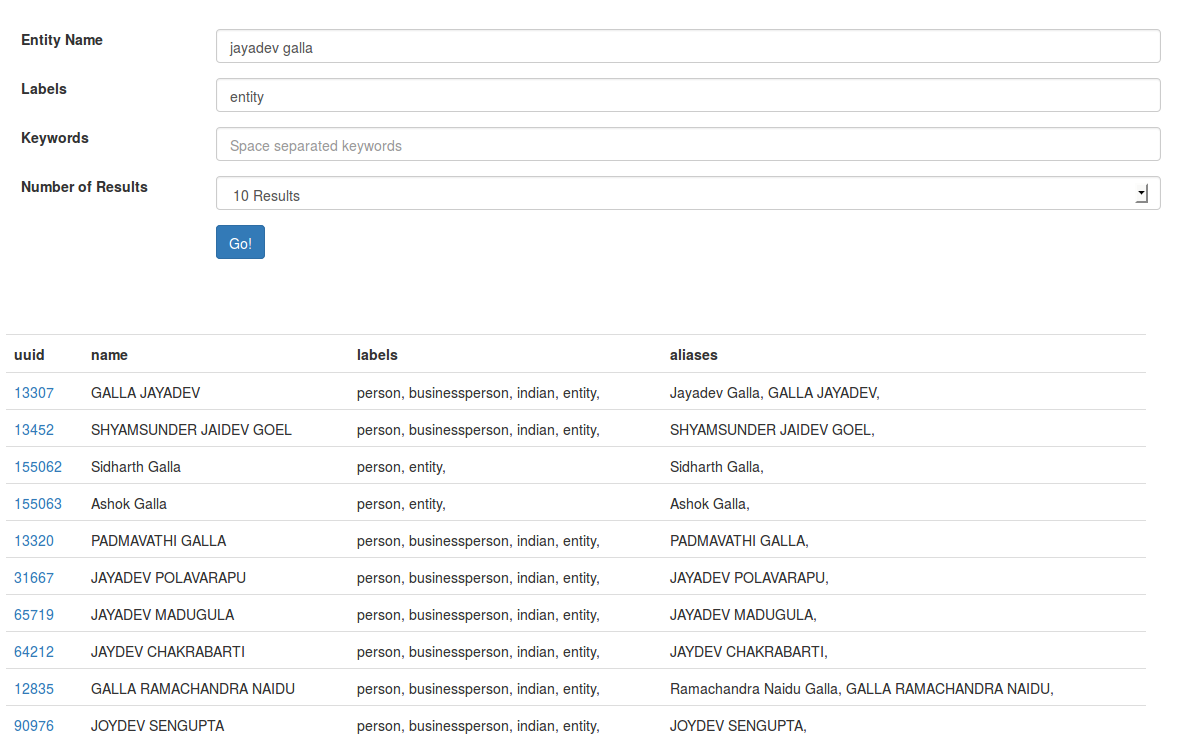
\includegraphics[scale=0.3]{endsearch} 
\caption{Search Page results}
\label{fig:endsearch}
\end{center}
\end{figure}


\item \textbf{View entity profiles and connections:} User can browse to profile pages of entities in our core data-store. The profile shows information about the particular entity and also displays first level relations for the same. An actual profile from the core data-store and connections for the same entity are shown in Figure \ref{fig:endprofile} and \ref{fig:endconnections} respectively.


\begin{figure}[H]
\begin{center}  
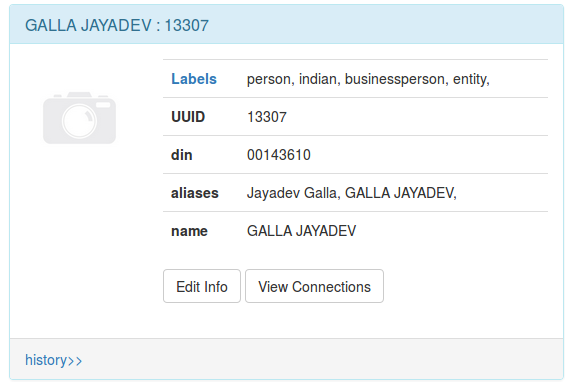
\includegraphics[width=0.6\textwidth]{endprofile} 
\caption{Entity profile from core data-store}
\label{fig:endprofile}
\end{center}
\end{figure}



\begin{figure}[H]
\begin{center}  
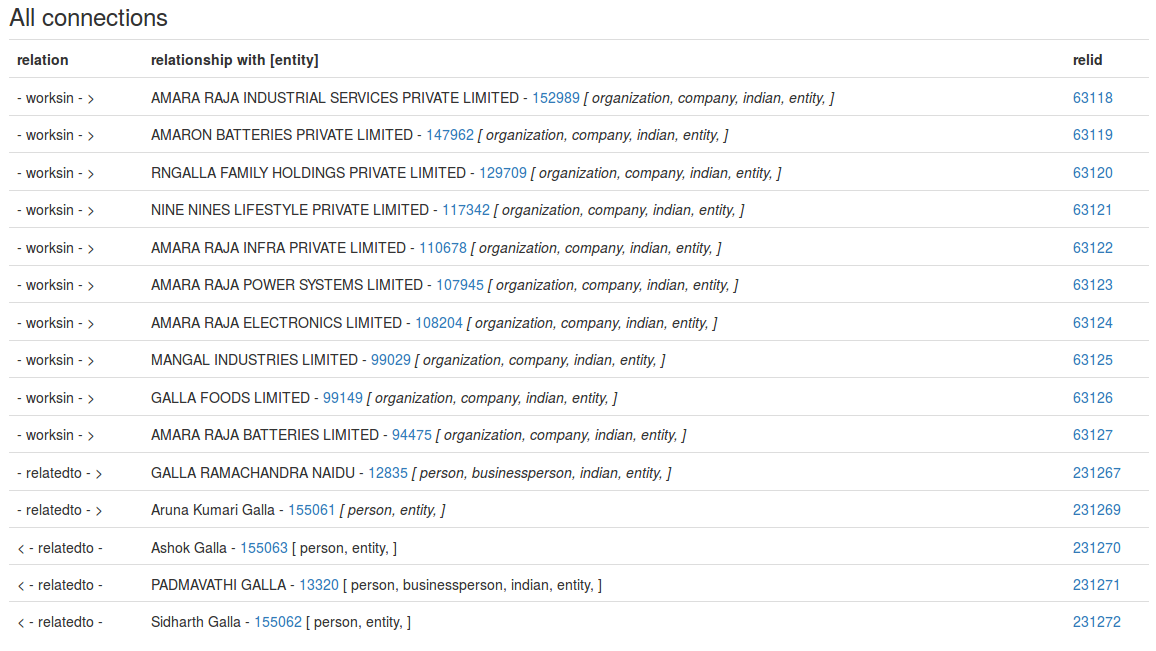
\includegraphics[scale=0.3]{endconnections} 
\caption{Entity connections from core data-store}
\label{fig:endconnections}
\end{center}
\end{figure}


\item \textbf{Visualizations for the end user:} The end user can generate visualizations for a cypher query. The cypher query is first validated for safety and load, and then executed. Result of an actual cypher query is shown in Figure \ref{fig:endviz}.

\begin{figure}[H]
\begin{center}  
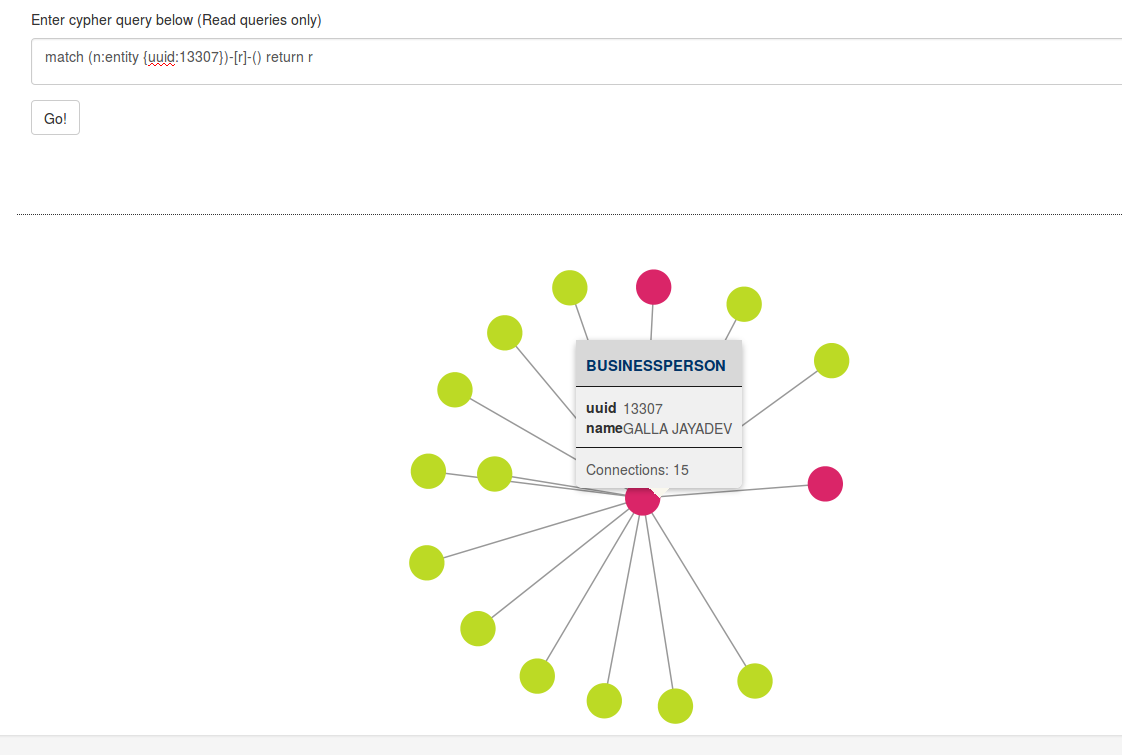
\includegraphics[width=1\textwidth]{endviz} 
\caption{End user generates visualization}
\label{fig:endviz}
\end{center}
\end{figure}


\end{enumerate}

% database model er diagrm sanphot meta db - index table also include?? [left] \\


\section{Admin}

\begin{enumerate}
    \item \textbf{Use Case:} Use case diagram for not logged in end users is shown in Figure \ref{fig:admin}.

    \begin{figure}[H]
    \begin{center}  
    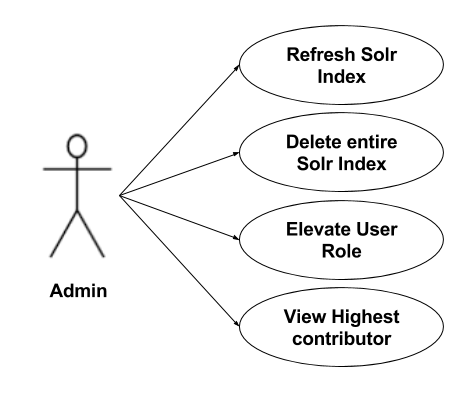
\includegraphics[scale=0.3]{admin} 
    \caption{Use cases for Admin}
    \label{fig:admin}
    \end{center}
    \end{figure}
    

     \item \textbf{Solr Indexes:} Admin can delete all the Solr indexes, and can also refresh them for maintenance purposes.

     \item \textbf{Change user roles:} Admin can change roles of existing authorized users, so a user roles in the system are always controlled by the admins.


     \item \textbf{View contributions:} Admin on a broader level needs to look over the verification/moderation process in the system. Towards that effect, an admin can view all the statistics about verifiers and data-gatherers present in the system.

     \item \textbf{Bots:} Not all the tasks can be done by humans alone, and thus we have introduced the concept of bots in the system. All these bots wake up at regular intervals and execute any background jobs scheduled for them. All these bots thus need to have admin roles for this purpose. We have a \emph{Location resolver bot} that periodically checks if any entity has an address field and is not connected to any city. It then automatically parses the address and introduces a relation from that entity to that city. We also have a \emph{Dangling locks release} bot that releases any dangling locks in the crawl data store after a specified interval.   

\end{enumerate}